\documentclass[11pt]{article}
\usepackage[parfill]{parskip}
\usepackage{graphicx}
\usepackage{wrapfig}
\usepackage{subcaption}
\usepackage[top=1in, bottom=1in, left=1in, right=1in]{geometry}
\bibliographystyle{plain}
\usepackage{amsmath}
\usepackage{hyperref}
%%%%%%%%%%%%%%%%%%%%%%%%%%%%%%%%%%%%%%%%%%%%%%%%%%%%%%%%%%%%%%%
\usepackage{fancyhdr}
\pagestyle{fancy}
%%% Please add the author's last names
\lhead{Davis, Theriault, Orhai, Westbrook, and Wright}
\rhead{Modeling the World's Systems, 2019}
%%% Please use \cfoot{} to remove page numbers
\cfoot{ }
\renewcommand{\headrulewidth}{0pt}
\renewcommand{\footrulewidth}{0pt}
%%%%%%%%%%%%%%%%%%%%%%%%%%%%%%%%%%%%%%%%%%%%%%%%%%%%%%%%%%%%%%&
\usepackage{titlesec}
\titlespacing{\section}{0pt}{\parskip}{-.5\parskip}
\titlespacing{\subsection}{0pt}{\parskip}{- .5\parskip}
\titlespacing{\subsubsection}{0pt}{\parskip}{- .5\parskip}
\newcommand{\closeup}{\setlength{\itemsep}{-4pt}}

\newcommand{\amidol}{\textsc{AMIDOL}}

\def\signed #1{{\leavevmode\unskip\nobreak\hfil\penalty50\hskip2em
  \hbox{}\nobreak\hfil(#1)%
  \parfillskip=0pt \finalhyphendemerits=0 \endgraf}}

\newsavebox\mybox
\newenvironment{aquote}[1]
  {\savebox\mybox{#1}\begin{quote}}
  {\signed{\usebox\mybox}\end{quote}}

\date{\vspace{-5ex}}
% Use this to get rid of the date

\usepackage{authblk}
\author[1]{Eric Davis}
\author[1]{Alec Theriault}
\author[1]{Max Orhai}
\author[1]{Eddy Westbrook}
\author[1]{Ryan Wright}
\affil[1]{Galois, Inc}

%\setcounter{page}{0}



\title{Machine-Assisted Extraction of Formal Semantics from Domain Specific Semi-Formal Diagrams}

\begin{document}
\maketitle
\vspace{10pt}
\begin{abstract}
Analyzing complex systems is a challenging process which requires not only teams of domain experts but often also a multidisciplinary team of data scientists, mathematicians, statisticians, and software engineers in order to support the life cycle of model development, model-based inference, as well as knowledge extraction and synthesis.  The models that typically result from this process today are bespoke, lack generalizability, are not performable, lack reusability, and are difficult to synthesize actionable knowledge and policies from their raw outputs.  In this paper we describe \amidol{}: the Agile Metamodel Inference using Domain-specific Ontological Languages, a project that aims to reduce the overhead associated with the development, deployment, maintenance, and reuse of models of complex systems.  Our technique utilizes a common intermediate representation which is designed to support a number of scientific, physical, social, and hybrid domains by allowing domain experts to define their models in novel ways, using domain specific ontological languages (VDSOLs).  The intermediate abstract representation provides formal, executable, meaning to the semi-formal diagrams domain experts normally create, and allow the inference engine to build prognostic queries on associated reward models.  \amidol{} binds results from the inference engine to the original ontologies providing more explainability when compared to conventional methods.
\end{abstract}

\section{Introduction}

The construction of computational models is an important practice for scientists, engineers, policy makers, and other domain experts as it provides a way to make formal predictions based on a formal expectation of system behavior, and allows practitioners to test hypotheses and explain phenomena in complex systems.  The process of building suitable models, however, is a laborious one which requires diverse teams of experts, significant manual effort, and typical results in models with severe limitations, low performability, and little reusability or generalizability.  Such models are not only costly to produce, both in time and effort, but are also prone to errors, difficult to verify, and do not utilize best practices in software development.

\amidol{} seeks to improve the problems inherent to modern machine-assisted inference with two high-level goals: 1) improving the ability of domain experts to build and maintain models and 2) improving the explainability and agility of the results of machine-inference.  The techniques applied to achieve these goals incorporate abstract intermediate representations, semantic knowledge representation and binding in graph structures, traditional machine learning and model solution techniques, with intuitive model generation giving meaning to the semi-formal diagrams already being generated by domain experts.

\begin{figure}
  \centering
  \begin{subfigure}[b]{0.48\textwidth}
    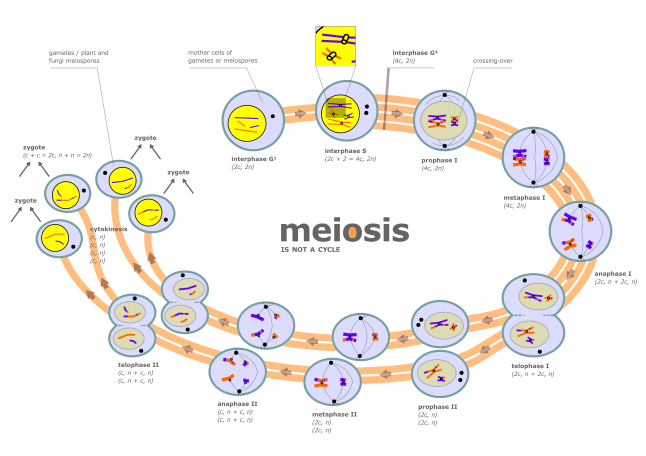
\includegraphics[width=\textwidth]{figs/Diagram_of_meiosis.pdf}
    \caption{Example of a semi-formal diagram of Meoisis. CC-BY-SA 3.0 Marek Kultys, July 2, 2008.}
    \label{Fig:Meiosis}
  \end{subfigure}
  \begin{subfigure}[b]{0.48\textwidth}
    \includegraphics[width=\textwidth]{figs/HIV-Tat-figure.pdf}
    \caption{Example of a semi-formal diagram of the molecular model of the Tat transactivation circuit.}
    \label{Fig:HIV-Tat}
  \end{subfigure}
  \caption{Examples of semi-formal diagrams drawn by domain experts to represent operational semantics and complex
  system models.}
  \label{Fig:Semi-formal}
\end{figure}

Current modeling formalisms are often specified in formal languages which seem arcane and unnatural to domain experts, but have unambigous formal meaning with defined execution semantics.  By contrast domain experts have naturally developed visual semi-formal ways of describing the systems they study, such as those indicated in Figure \ref{Fig:Semi-formal}, but which lack semantic meaning, executability, and are often ambiguous.

\begin{eqnarray}
\frac{d\ tat}{dt} &=& -dtt \cdot tat\\
\frac{d\ nRNA}{dt} &=& \frac{(b + v \cdot tat)}{k + tat} - ex \cdot nRNA - dr \cdot nRNA\\
\frac{d\ cRNA}{dt} &=& ex \cdot nRNA - dr \cdot cRNA\\
\frac{d\ P}{dt} &=& \frac{vp \cdot cRNA}{kp + cRNA} - dp \cdot P
\end{eqnarray}
 
\begin{aquote}{\cite{nurse2008life} Paul Nurse (2008)}
"There should be
a concerted programme \ldots which will require both the development of
the appropriate languages to describe information processing in biological systems and the generation of more effective methods to
translate biochemical descriptions into the
functioning of the logic circuits that underpin
biological phenomena."
\end{aquote}

Abstract machines of systems biology \cite{cardelli2005abstract}

\paragraph{Significance}

\section{Related Work}

Gene gate modeling in the stochastic pi-calculus \cite{blossey2008compositionality}

State charts \cite{harel1987statecharts}

Pi-calculus \cite{sangiorgi2003pi}

Petri-net modeling of biological networks \cite{chaouiya2007petri}

\subsection{Generating Formal Meaning from Informal Diagrams}

\section{AMIDOL}

\begin{figure}
  \includegraphics[width=\textwidth]{figs/system-architecture-quad.pdf}
  \caption{AMIDOL Architecture}
\end{figure}

\subsection{Visual Domain Specific Languages}

Composition \cite{sanders1992dependability,sanders1988construction}

\subsection{Intermediate Representation}

Markov models \cite{howard2012dynamic}

Petri-nets with inhibitor arcs \cite{chiola1993generalized}

Stochastic activity networks \cite{movaghar1985performability,sanders2000stochastic}

\paragraph{State and reward variables}

Reward structures \cite{qureshi1996algorithms,deavours1999efficient,ciardo1996well,sanders1991reduced}

Instant of time... \cite{freire1990technique}

\paragraph{Events}

\paragraph{Input and output predicates}

\subsection{Inference Engine}

\begin{figure}
  \includegraphics[width=\textwidth]{figs/table.pdf}
  \caption{}
  \label{Fig:InferenceClasses}
\end{figure}

\section{Compartmental Model for Epidemiology}

\subsection{SIRS Model}

H1N1 $R_0$ importance \cite{fraser2009pandemic}.

Ebola $R_0$ importance \cite{fisman2014early}

CDC Data \cite{cdc2019fluview}

\subsection{Vital Dynamics}

\section{Conclusions}

\section{Future Work}

\section{Acknowledgments}

This research has been supported by DARPA contract DARPA-PA-18-02-AIE-FP-039.

\section{Resources, web sites, etc.}

MWS seeks to build a community and share resources, so feel free to have a section in your paper that points readers to web sites, github pages, etc.


%\newcommand*{\doi}[1]{\href{http://dx.doi.org/#1}{doi: #1}}
\bibliography{AMIDOL-MWS}



\end{document}
